\tableofcontents
\section*{Предисловие}
При выполнении данной лабораторной работы было решено использовать 
\href{https://python-control.readthedocs.io/en/0.9.4/}{Python Control Systems Library}.
Данный инструмент является альтернативой Matlab, адаптированной для использования на 
языке Python и предоставляет широкий функционал для анализа и моделирования систем,
а также синтеза регуляторов для управления.

Полный листинг моделирования систем представлен в \href{https://github.com/diuzhevVlad/control-theory-itmo-fall-2023/blob/main/Lab7/Lab7.ipynb}{jupyter notebook} на GitHub.

\pagebreak

\section{Модальный регулятор}
Рассмотрим систему:
\begin{equation}
    \dot{x} = Ax + Bu
\end{equation}
Матрицы $A$ и $B$:
\begin{equation*}
    A = \begin{bmatrix}
        -1 & 0 & 0 & 0 \\
        0 & 2 & 0 & 0 \\
        0 & 0 & 3 & 4 \\
        0 & 0 & -4 & 2
    \end{bmatrix},
    B = \begin{bmatrix}
        0 \\ 5 \\ 0 \\ 6
    \end{bmatrix}
\end{equation*}
Матрица $A$ представлена в Жордановой форме, значит ее спектр:
\begin{equation*}
    \sigma (A) = \{-1,2,3-4i, 3+4i\}
\end{equation*}
Заметим, что все собственные числа, кроме $-1$ являются управляемыми. Следовательно система -- частично управляема и стабилизируема.

Для задания желаемого спектра матрице $A + B \cdot K$ необходимо выбрать $K$, таким образом, чтобы
она была подобна задаваемой матрице $G$ (имеющей желаемый спектр).
\begin{equation}
    A + BK = PGP^{-1} \implies AP - PG = -BKP
\end{equation}
\begin{equation*}
    Y = -KP \implies AP - PG = BY 
\end{equation*}
Задав матрицу $Y$, можем решить уравнение Сильвестра и найти $P$. Затем, выразим $K$:
\begin{equation}
    K = -YP^{-1}
\end{equation}

Согласно варианту, желаемые спектры имеют вид:
\begin{equation*}
    \sigma_1 = \{-1,-1,-1,-1\}, \sigma_2 = \{-1,-10,-100,-100\}, 
\end{equation*}
\begin{equation*}
    \sigma_3 = \{-1,-10,4i,-4i\}, \sigma_4 = \{-1,-10,-3+4i,-3-4i\}
\end{equation*}
Соответствующие им матрицы:
\begin{equation*}
    G_1 = \begin{bmatrix}
        -1 & 1 & 0 & 0 \\
        0 & -1 & 1 & 0 \\
        0 & 0 & -1 & 1 \\
        0 & 0 & 0 & -1
    \end{bmatrix},
    G_2 = \begin{bmatrix}
        -1 & 0 & 0 & 0 \\
        0 & -10 & 0 & 0 \\
        0 & 0 & -100 & 1 \\
        0 & 0 & 0 & -100
    \end{bmatrix},
\end{equation*}
\begin{equation*}
    G_3 = \begin{bmatrix}
        -1 & 0 & 0 & 0 \\
        0 & -10 & 0 & 0 \\
        0 & 0 & 0 & 4 \\
        0 & 0 & -4 & 0
    \end{bmatrix},
    G_4 = \begin{bmatrix}
        -1 & 0 & 0 & 0 \\
        0 & -10 & 0 & 0 \\
        0 & 0 & -3 & 4 \\
        0 & 0 & -4 & -3
    \end{bmatrix}
\end{equation*}
Матрицу $Y$ выберем следующим образом (первое собственное число не управляемо):
\begin{equation*}
    Y = \begin{bmatrix}
        0 & 1 & 1 & 1
    \end{bmatrix}
\end{equation*}

Для каждого желаемого спектра найдем матрицу $K$ и выполним моделирование системы с 
входным воздействием $u = Kx$ при начальных условиях $x(0)=[1, 1, 1, 1]^T$.

\begin{figure}[]
    \centering
    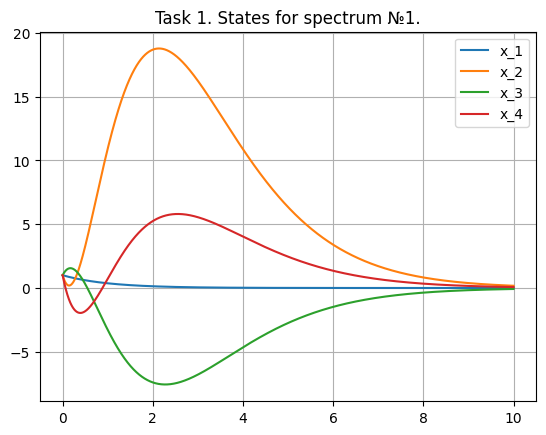
\includegraphics[width=300px]{plot_1_st_1.png}
    \caption{\label{fig:The-caption-1}Задание 1. Компоненты вектора состояний системы со спектром №1}
\end{figure}
\begin{figure}[]
    \centering
    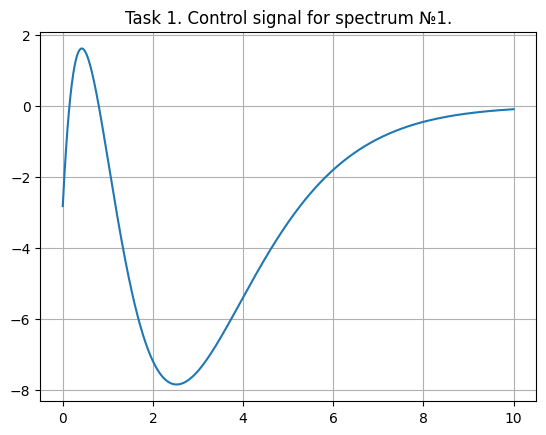
\includegraphics[width=300px]{plot_1_ct_1.png}
    \caption{\label{fig:The-caption-1}Задание 1. Управляющий сигнал системы со спектром №1}
\end{figure}
\begin{figure}[]
    \centering
    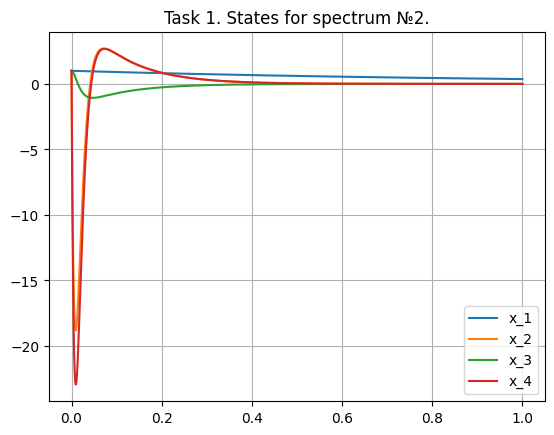
\includegraphics[width=300px]{plot_1_st_2.png}
    \caption{\label{fig:The-caption-1}Задание 1. Компоненты вектора состояний системы со спектром №2}
\end{figure}
\begin{figure}[]
    \centering
    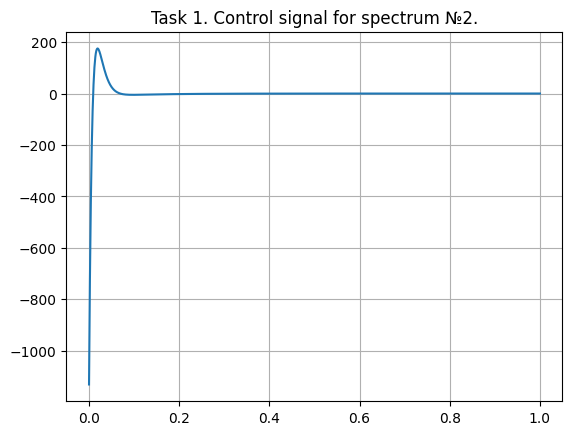
\includegraphics[width=300px]{plot_1_ct_2.png}
    \caption{\label{fig:The-caption-1}Задание 1. Управляющий сигнал системы со спектром №2}
\end{figure}
\begin{figure}[]
    \centering
    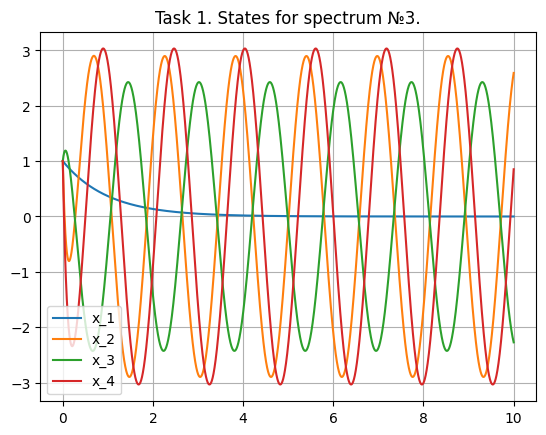
\includegraphics[width=300px]{plot_1_st_3.png}
    \caption{\label{fig:The-caption-1}Задание 1. Компоненты вектора состояний системы со спектром №3}
\end{figure}
\begin{figure}[]
    \centering
    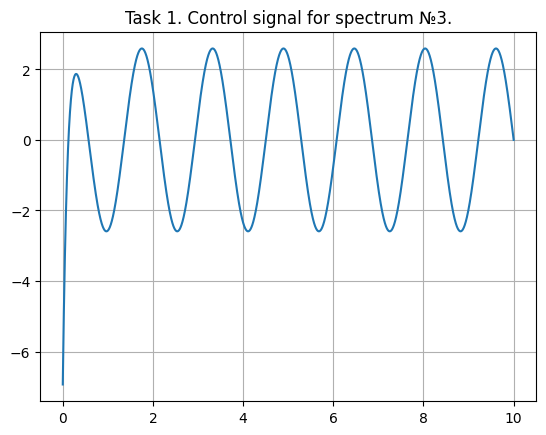
\includegraphics[width=300px]{plot_1_ct_3.png}
    \caption{\label{fig:The-caption-1}Задание 1. Управляющий сигнал системы со спектром №3}
\end{figure}
\begin{figure}[]
    \centering
    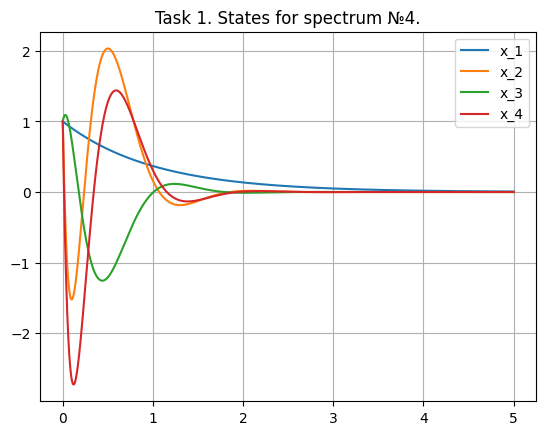
\includegraphics[width=300px]{plot_1_st_4.png}
    \caption{\label{fig:The-caption-1}Задание 1. Компоненты вектора состояний системы со спектром №4}
\end{figure}
\begin{figure}[]
    \centering
    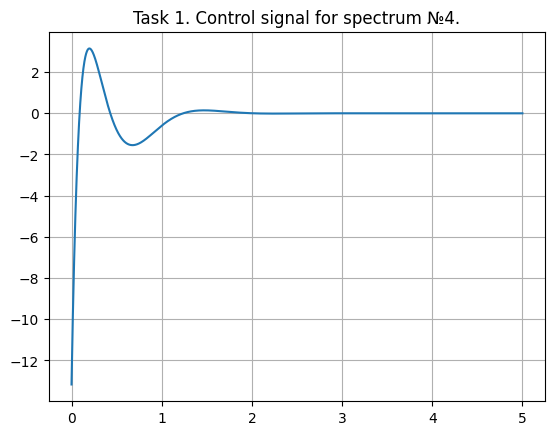
\includegraphics[width=300px]{plot_1_ct_4.png}
    \caption{\label{fig:The-caption-1}Задание 1. Управляющий сигнал системы со спектром №4}
\end{figure}
\pagebreak

\section{Модальный наблюдатель}
Рассмотрим систему:
\begin{equation}
    \dot{x} = Ax, y = Cx
\end{equation}
Матрицы $A$ и $B$:
\begin{equation*}
    A = \begin{bmatrix}
        0 & 3 & 0 & 0 \\
        -3 & 0 & 0 & 0 \\
        0 & 0 & 0 & 1 \\
        0 & 0 & -1 & 0
    \end{bmatrix},
    C = \begin{bmatrix}
        2 & 0 & 0 & 3
    \end{bmatrix}
\end{equation*}
Матрица $A$ представлена в Жордановой форме, значит ее спектр:
\begin{equation*}
    \sigma (A) = \{-3i,3i,-i,i\}
\end{equation*}
Заметим, что все собственные числа являются наблюдаемыми. Следовательно система -- наблюдаема.

Рассмотрим систему:
\begin{equation}
    \dot{\hat x} = A\hat x + L(\hat y - y), \hat y = C\hat x
\end{equation}
Введем величну ошибки наблюдателя $e(t)=x(t)-\hat x(t)$:
\begin{equation}
    \dot e = Ae + LCe
\end{equation}
Заметим, что задав спектр матрицы, $A + LC$, представив подобную ей, можем определить тип переходного процесса ошибки наблюдателя.
\begin{equation}
    A+LC = Q^{-1}GQ \implies GQ - QA = YC, Y = -QL 
\end{equation}
Выбрав $Y$ и решив уравнение Сильвестра из выражения (7), можем найти матрицу $L$.

Желаемые спектры матрицы $A + LC$ совпадают с указанными в первом задании (матрицы $G$, соответственно, тоже).
Матрицу Y выберем следующим образом:
\begin{equation*}
    Y = \begin{bmatrix}
        1 \\ 1 \\ 1 \\ 1
    \end{bmatrix}
\end{equation*}


Для каждого желаемого спектра найдем матрицу $L$ и выполним моделирование при начальных
условиях $x(0)=[1, 1, 1, 1]^T$, $\hat x(0)=[2, 0, 0, -1]^T$.

\begin{figure}[]
    \centering
    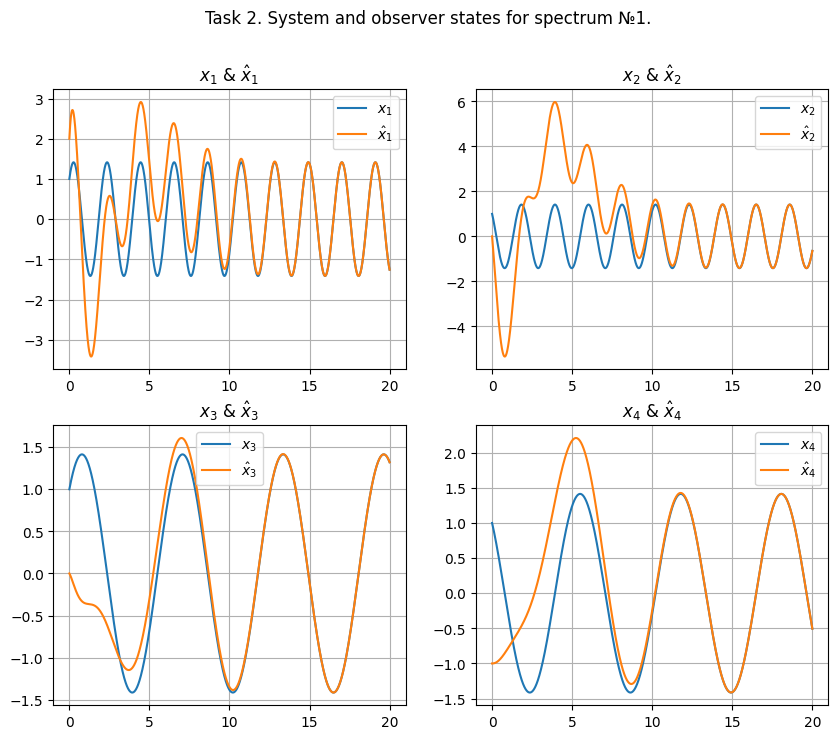
\includegraphics[width=300px]{plot_2_st_1.png}
    \caption{\label{fig:The-caption-1}Задание 2. Компоненты вектора состояний системы со спектром №1}
\end{figure}
\begin{figure}[]
    \centering
    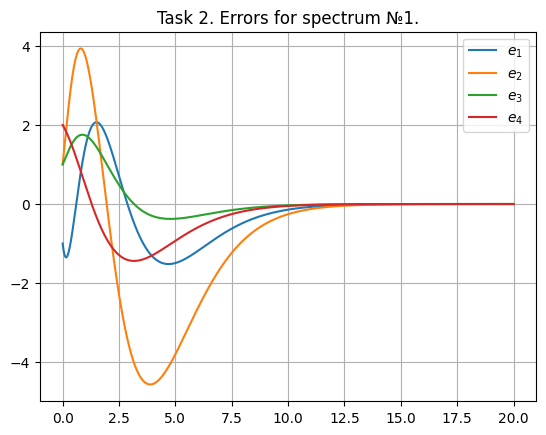
\includegraphics[width=300px]{plot_2_err_1.png}
    \caption{\label{fig:The-caption-1}Задание 2. Ошибка наблюдателя системы со спектром №1}
\end{figure}
\begin{figure}[]
    \centering
    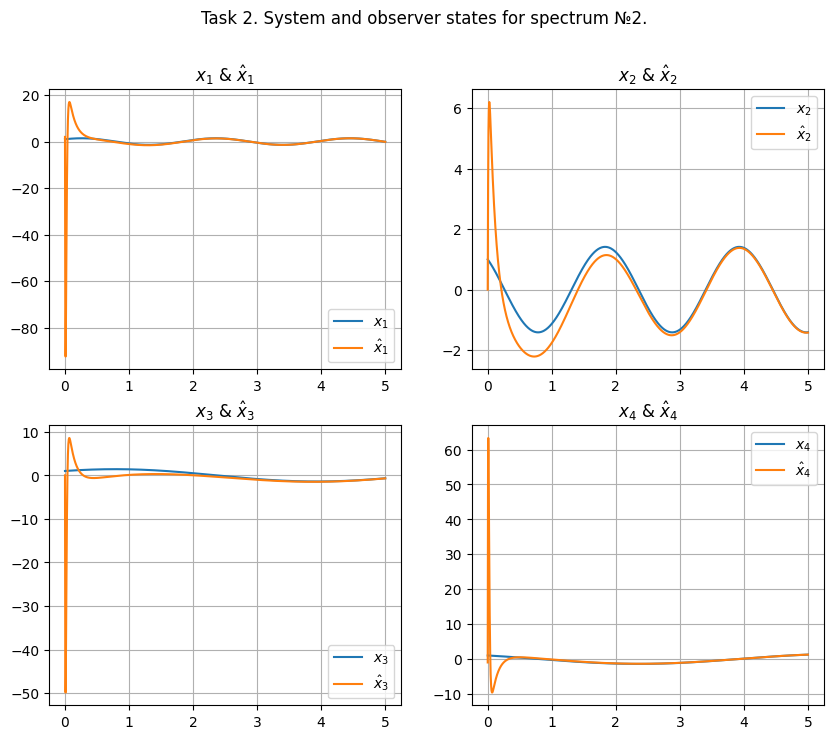
\includegraphics[width=300px]{plot_2_st_2.png}
    \caption{\label{fig:The-caption-1}Задание 2. Компоненты вектора состояний системы со спектром №2}
\end{figure}
\begin{figure}[]
    \centering
    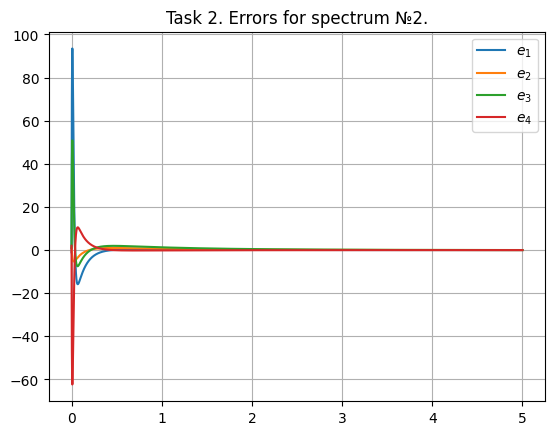
\includegraphics[width=300px]{plot_2_err_2.png}
    \caption{\label{fig:The-caption-1}Задание 2. Ошибка наблюдателя системы со спектром №2}
\end{figure}
\begin{figure}[]
    \centering
    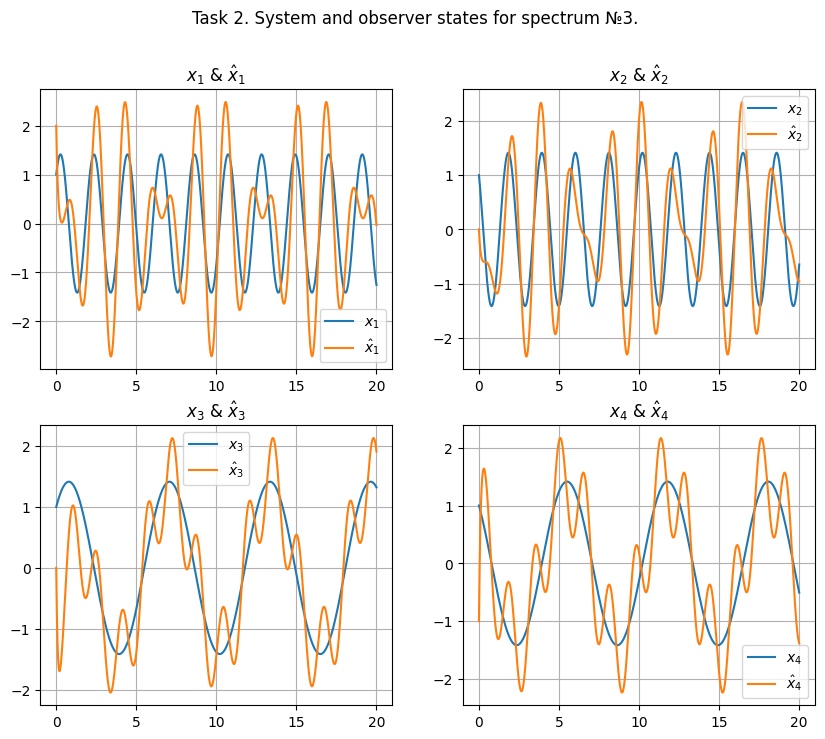
\includegraphics[width=300px]{plot_2_st_3.png}
    \caption{\label{fig:The-caption-1}Задание 2. Компоненты вектора состояний системы со спектром №3}
\end{figure}
\begin{figure}[]
    \centering
    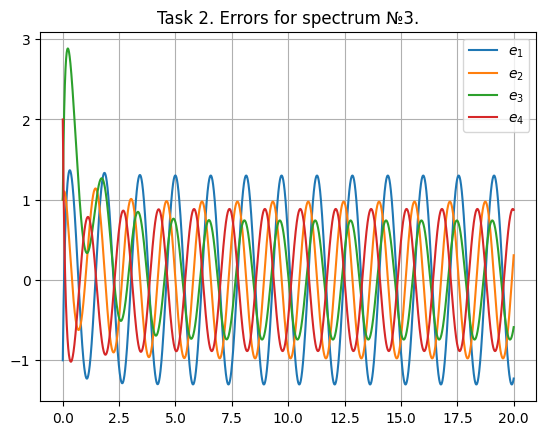
\includegraphics[width=300px]{plot_2_err_3.png}
    \caption{\label{fig:The-caption-1}Задание 2. Ошибка наблюдателя системы со спектром №3}
\end{figure}
\begin{figure}[]
    \centering
    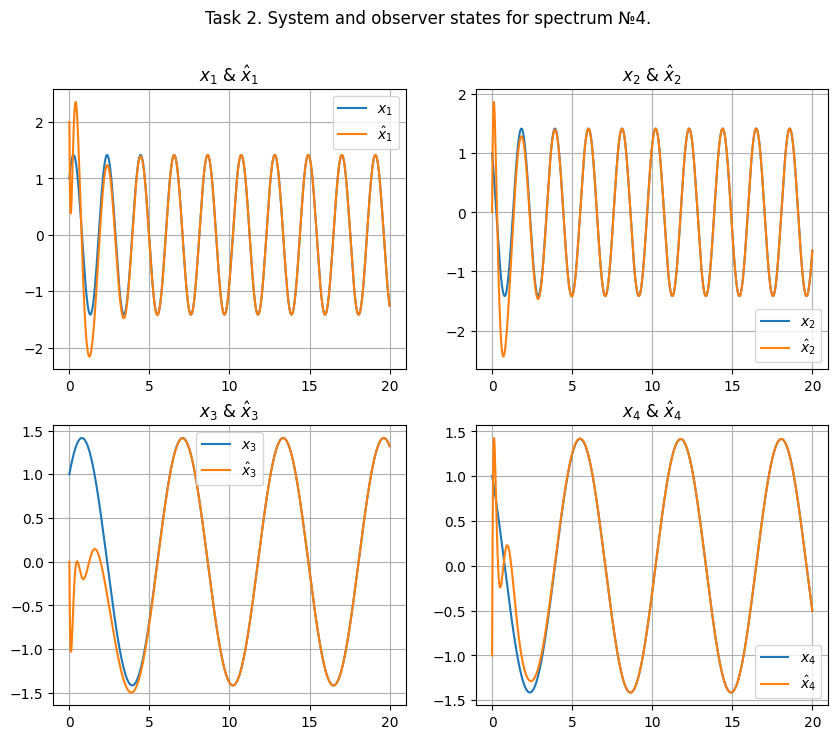
\includegraphics[width=300px]{plot_2_st_4.png}
    \caption{\label{fig:The-caption-1}Задание 2. Компоненты вектора состояний системы со спектром №4}
\end{figure}
\begin{figure}[]
    \centering
    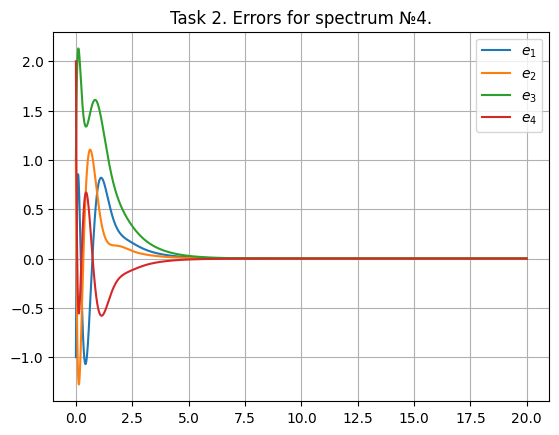
\includegraphics[width=300px]{plot_2_err_4.png}
    \caption{\label{fig:The-caption-1}Задание 2. Ошибка наблюдателя системы со спектром №4}
\end{figure}

\pagebreak

\section{Регулятор + наблюдатель}
Рассмотрим систему:
\begin{equation}
    \begin{cases}
        \dot x = Ax + Bu \\
        y = Cx
    \end{cases}
\end{equation}
Матрицы $A$, $B$ и $C$:
\begin{equation*}
    A = \begin{bmatrix}
        3 & -11 & -7 & 5 \\
        -11 & 3 & -5 & 7 \\
        -7 & -5 & 3 & 11 \\
        5 & 7 & 11 & 3
    \end{bmatrix},
    B = \begin{bmatrix}
        2 \\ 4 \\ 2 \\ 4
    \end{bmatrix},
    C = \begin{bmatrix}
        3 & -2 & 2 & 2 \\
        2 & 4 & -2 & 4
    \end{bmatrix}
\end{equation*}
Жорданова форма матрицы $A$:
\begin{equation*}
    A = PJP^{-1}, J = diag(\{-20,4,12,16\})
\end{equation*}
При этом:
\begin{equation*}
    P^{-1}B = \begin{bmatrix}
        -1\\2\\1\\2
    \end{bmatrix},
    CP= \begin{bmatrix}
        0 & 0 & 8 & 0 \\
        0 & 12 & 0 & 4
    \end{bmatrix}
\end{equation*}
Можем сделать вывод, что система является полностью управляемой, однако частично наблюдаемой 
(собственное число -20 не является наблюдаемым). При этом система обнаруживаема.

Построим регулятор, состоящий из наблюдателя $\dot{\hat x} = A\hat x + Bu + L(C\hat x - y)$,
где $u = K\hat x$. Матрицы $K$ и $L$ можем найти независимо, согласно алгоритмам, рассмотренным
в прошлых заданиях. Матрицы $Y$ для этого выберем следующим образом:
\begin{equation*}
    Y_K = \begin{bmatrix}
        1 & 1 & 1 & 1
    \end{bmatrix},
    Y_L = \begin{bmatrix}
        0 & 0 \\
        1 & 1 \\
        1 & 1 \\
        1 & 1
    \end{bmatrix}
\end{equation*}
Желаемый спектр матриц $A + BK$ и $A + LC$ примем равным $\sigma=\{-10,-11,-12,-13\}$.
Соответствующая матрица $G=diag(\sigma)$.

Можем представить систему в виде приведенной матрицы (имеющей блочно-треугольный вид):
\begin{equation}
    \tilde{A} = \begin{bmatrix}
        A + BK & -BK \\
        \Theta & A + LC
    \end{bmatrix}
\end{equation}

Вполним моделирование данной системы.
\begin{figure}[]
    \centering
    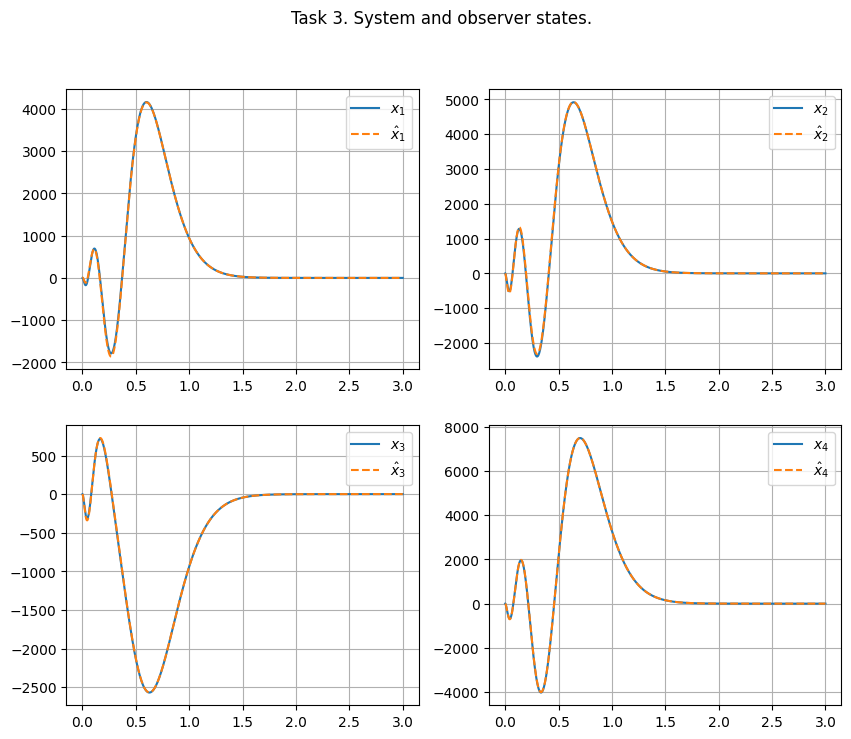
\includegraphics[width=300px]{plot_3_st.png}
    \caption{\label{fig:The-caption-1}Задание 3. Компоненты вектора состояний исходной системы и наблюдателя.}
\end{figure}
\begin{figure}[]
    \centering
    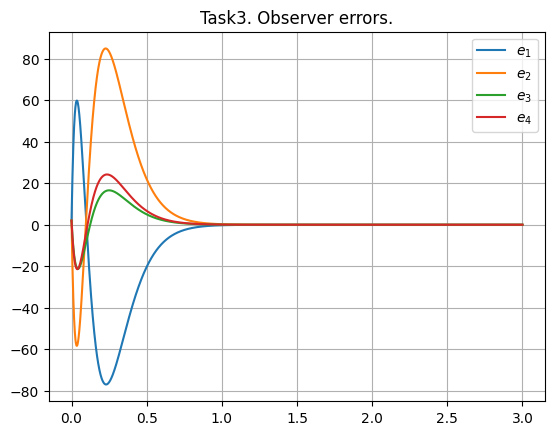
\includegraphics[width=300px]{plot_3_err.png}
    \caption{\label{fig:The-caption-1}Задание 3. Ошибка наблюдателя системы.}
\end{figure}
\begin{figure}[]
    \centering
    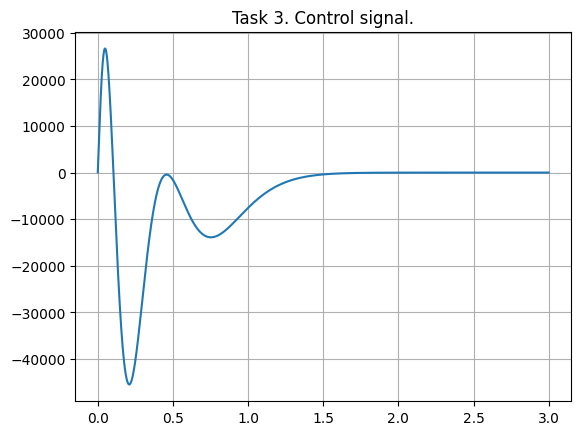
\includegraphics[width=300px]{plot_3_ct.png}
    \caption{\label{fig:The-caption-1}Задание 3. управляющий сигнал системы.}
\end{figure}
\begin{figure}[]
    \centering
    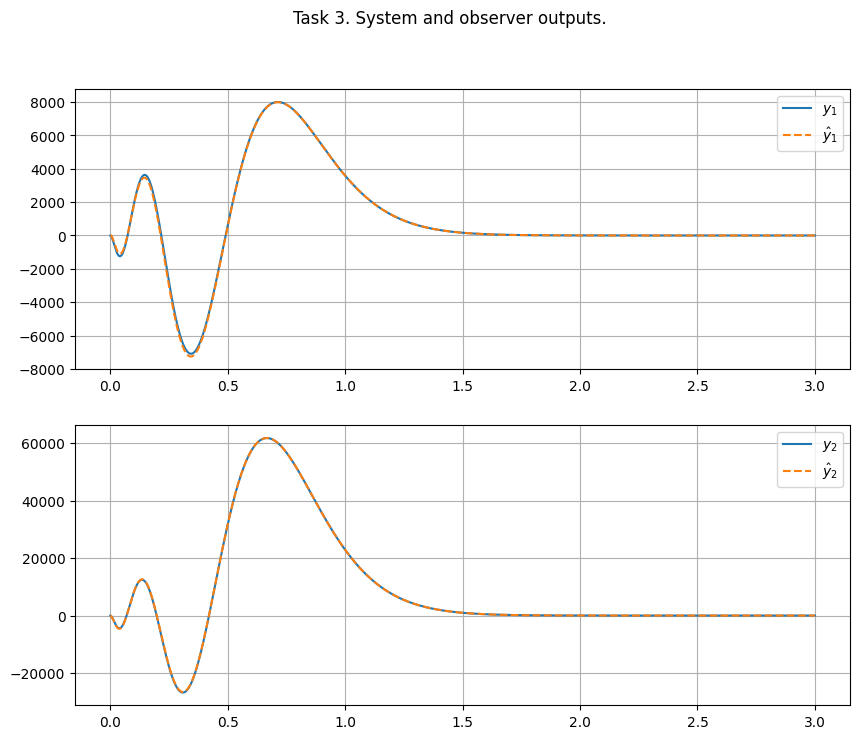
\includegraphics[width=300px]{plot_3_y.png}
    \caption{\label{fig:The-caption-1}Задание 3. Выходное воздействие системы и наблюдателя.}
\end{figure}
\pagebreak

\section{Выводы}
В ходе выполнения данной лабораторной работы удалось получить навыки синтеза модальных регуляторов
и наблюдателей для линейных систем. В ходе выполнения заданий, заметим:
\begin{enumerate}
    \item Характер переходных процессов вектора состояний наблюдался согласно выбранному спектру.
    \item Характер переходных процессов ошибки наблюдателя наблюдался согласно выбранному спектру.
    \item Характер переходных процессов вектора состояний системы и ошибки наблюдателя наблюдался согласно выбранному спектру.
\end{enumerate}
При синтезе модальных регуляторов и наблюдателей важную роль играет выбор вспомогательных матриц
$Y_K$ и $Y_L$.